\meutodo{
  Experimentos:
  - Descrição das bases
  - Descrição das ferramentas/técnicas/pacotes
  - Descrição do protocolo
  - Apresentação dos resultados
  - Discussão dos resultados
}

\meutodo{
  Qual adição de ruído? Qual nível?
}

\meutodo{
  Variação gradual de parâmetros para identificar o que causa perdas/ganhos
}

%--------------------------------------------------------------------------------
\section{Considerações iniciais}

Este capítulo apresenta os resultados preliminares obtidos. Primeiramente, é apresentada a descrição do experimento realizado, ressaltando os métodos de extração de características, quantização e classificação utilizados. Além disso, o fluxo de operações para a realização do experimento é descrito. Em seguida, os resultados são propriamente ilustrados, ao indicar que a geração de imagens artificiais é promissora para o cenário de bases desbalanceadas. Por fim, as atividades futuras são destacadas.

%--------------------------------------------------------------------------------
\section{Descrição do experimento}

Algumas pesquisas sobre os efeitos da sobreamostragem e geração de exemplos artificiais em dados de aprendizado de máquina já foram realizadas~\cite{Kuncheva2004,Chawla2002}. O método mais divulgado na literatura é conhecido como SMOTE (\textit{Synthetic Minority Over-sampling Technique}). Este método propõe a geração de exemplos artificiais a partir dos vetores de características originais das classes minoritárias. Não há registro conhecido de um estudo dessas técnicas em dados de informação visual para o rebalanceamento de classes.

% \enlargethispage{-\baselineskip}

Assim, foi proposta a geração de novas imagens a partir de operações como adição de ruído, borramento, mistura e combinação das imagens originais. Tais operações estão exemplificadas na Figura~\ref{fig:ArtificialImages}, utilizando a classe ``praia'' da base de imagens naturais COREL-1000. A partir das imagens originais --- primeira linha da figura --- são geradas imagens artificiais por meio das operações citadas, resultando nas imagens da segunda linha da figura.

\vspace{25pt}

\renewcommand{\tabcolsep}{0.04cm}
\begin{figure}[!h]
 \begin{center}
 \begin{tabular}{ccccc}
   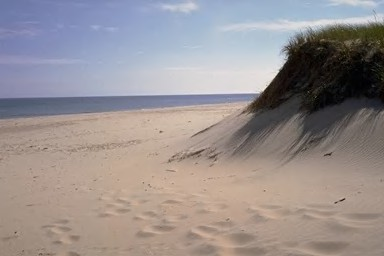
\includegraphics[width=0.245\linewidth]{\detokenize {figuras/original-1.jpg}}&
   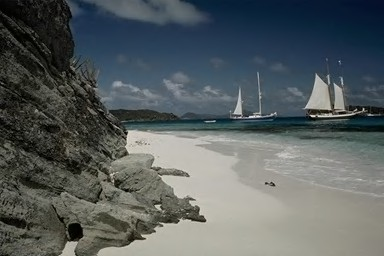
\includegraphics[width=0.245\linewidth]{\detokenize {figuras/original-2.jpg}}&
   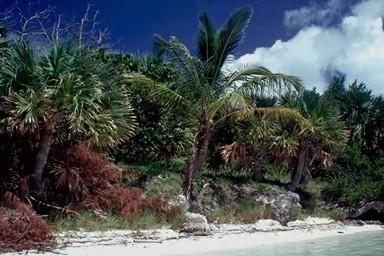
\includegraphics[width=0.245\linewidth]{\detokenize {figuras/original-3.jpg}}&
   % 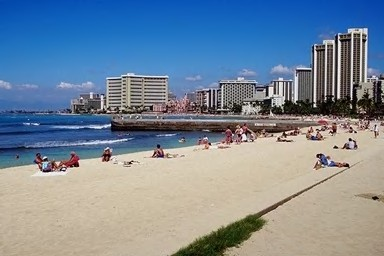
\includegraphics[width=0.19\linewidth]{\detokenize {figuras/original-4.jpg}}&
   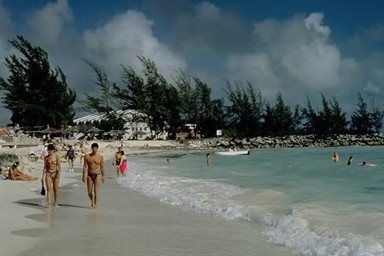
\includegraphics[width=0.245\linewidth]{\detokenize {figuras/original-5.jpg}}\\
   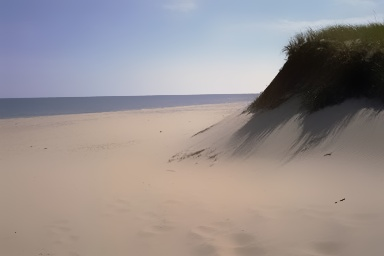
\includegraphics[width=0.245\linewidth]{\detokenize {figuras/gerada-1_blur.jpg}}&
   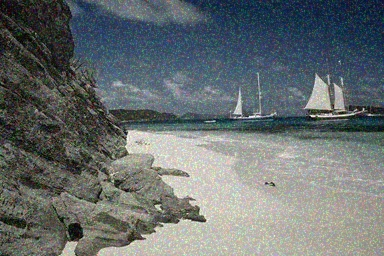
\includegraphics[width=0.245\linewidth]{\detokenize {figuras/gerada-2_ruido.jpg}}&
   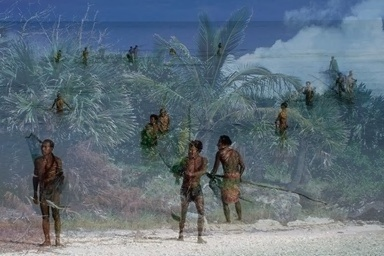
\includegraphics[width=0.245\linewidth]{\detokenize {figuras/gerada-3_blend.jpg}}&
   % 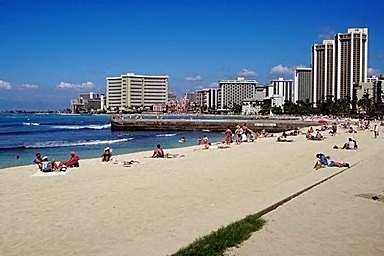
\includegraphics[width=0.19\linewidth]{\detokenize {figuras/gerada-4_unsharpMask.jpg}}&
   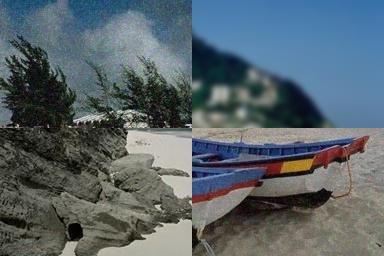
\includegraphics[width=0.245\linewidth]{\detokenize {figuras/gerada-5.jpg}} \\
 \end{tabular}
 \end{center}
  \caption[Geração de imagens artificiais para o rebalanceamento de classes.]{Geração de imagens artificiais para o rebalanceamento de classes. A partir das imagens originais mostradas na primeira linha, são geradas imagens artificiais por meio de: borramento, adição de ruído, mistura e combinação. Os resultados dessas operações estão demonstrados na segunda linha, em ordem. \textit{Fonte:~Elaborado pelo autor.}}
 \label{fig:ArtificialImages}
\end{figure}
\renewcommand{\tabcolsep}{0.5cm}
\vspace{25pt}


Os descritores de características utilizados para os resultados foram apresentados na Seção \ref{sec:extracao}. \todo{qual experimento anterior? explicar!} Considerando que em um experimento anterior o melhor resultado foi atribuído à quantização com o método de Intensidade para o extrator Haralick e MSB para os outros, apenas esses testes foram aprofundados (tópico anteriormente discutido na Seção \ref{sec:quantizacao}). Neste experimento, o classificador KNN foi utilizado, com $K=1$. Inicialmente o classificador Naive Bayes foi explorado, apresentando melhora na acurácia ao apenas replicar as imagens. Esse comportamento não é desejado em um classificador para a avaliação de rebalanceamento de classes. O código desenvolvido para esses resultados preliminares está disponível em \url{https://bitbucket.org/moacirponti/imagefeatureextraction/overview}.


%--------------------------------------------------------------------------------
\subsection{Fluxo de operações}

Para a realização desse experimento, iniciou-se com uma base originalmente balanceada e foram realizadas as seguintes operações:

\begin{enumerate}
\item Diminuir logaritmicamente o número de imagens de uma das classes, de modo a obter uma base desbalanceada;
\item Para cada estágio de desbalanceamento, realizar três experimentos:
\begin{enumerate}
\item A classificação direta, sem nenhuma operação de rebalanceamento;
\item A operação de SMOTE, após a extração de características e antes da classificação;
\item Rebalanceamento da classe minoritária com a geração de imagens antes da extração de características.
\label{item}
\end{enumerate}
\item Extrair as características com os descritores: ACC, BIC, CCV, GCH e Haralick6; e os quantizadores: Intensidade, Gleam, Luminância e MSB;
\item Classificar com KNN utilizando validação cruzada por \textit{repeated random-subsampling};
\item Executar os passos de 2 a 4 no mínimo 10 vezes para cada par de extrator e quantizador;
\item Calcular a matriz de confusão, a acurácia balanceada, a medida-F e o teste de Friedman para os resultados encontrados;
\item Gerar os gráficos para visualização dos resultados.
\end{enumerate}

%--------------------------------------------------------------------------------
\subsection{Geração das imagens artificiais}

As etapas para a geração das imagens artificiais, passo \ref{item} da seção anterior, foram:

\begin{enumerate}
\item Particionar a classe minoritária em conjuntos de treino e teste;
\item Selecionar uma imagem aleatoriamente do conjunto de treino;
\item Selecionar uma operação aleatória entre: borramento, adição de ruído, \textit{unsharp mask}, mistura ou composição;
\begin{enumerate}
\item Caso seja selecionada a composição: encontrar uma outra imagem aleatória, selecionar um quadrante dessa imagem e novamente uma operação entre: borramento, adição de ruído, \textit{unsharp mask} ou mistura;
\end{enumerate}
\item Aplicar essa operação na imagem previamente selecionada e adicionar essa imagem gerada ao conjunto de treino;
\item Repetir os passos 2 a 4 até que as classes estejam igualmente balanceadas.
\end{enumerate}

%--------------------------------------------------------------------------------
\section{Resultados}
\label{sec:resultadospreliminares}

Este estudo preliminar apresentou evidências experimentais de que, em problemas de duas classes (apresentadas na Figura~\ref{fig:praiamontanha}), pode haver ganho estatístico da medida-F ao gerar imagens, quando comparado à geração de exemplos artificiais no espaço de atributos (ou seja, depois que as características já foram extraídas das imagens). Essa melhoria pode ser notada na Figura~\ref{fig:resultmelhor}, que apresenta a relação da medida-F com a taxa de balanceamento, utilizando: as imagens originais, a geração de exemplos com SMOTE e as imagens geradas. Para essa configuração, foi utilizado o descritor de características ACC com a conversão em escala de cinza por MSB e a operação de pré-processamento por combinação. As classes ``praia'' e ``montanha'' foram escolhidas por serem as classes que possuem maior dificultade de diferenciação, havendo alta taxa de sobreposição de intensidades de cores e texturas, conforme testes realizados.

\vspace{20pt}

\begin{figure}[!htb]
 \begin{center}
   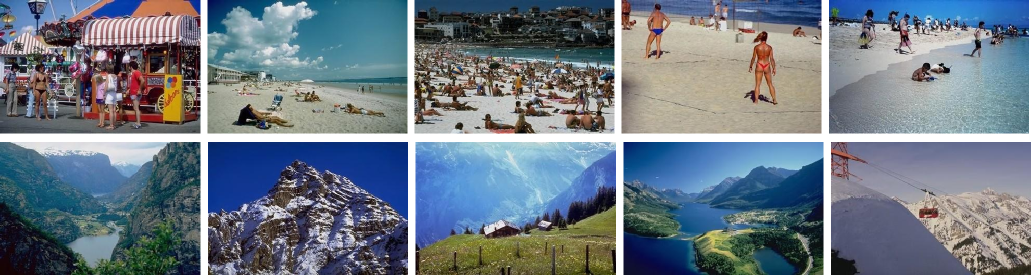
\includegraphics[width=\linewidth]{\detokenize {figuras/praia-montanha.png}}
 \end{center}
  \caption[Classes ``praia'' e ``montanha'' da base de imagens COREL-1000.]{Classes ``praia'' (primeira linha) e ``montanha'' (segunda linha) da base de imagens COREL-1000. \textit{Fonte:~Elaborado pelo autor.}}
 \label{fig:praiamontanha}
\end{figure}

\vspace{10pt}

\begin{figure}[!hbpt]
 \begin{center}
\begin{subfigure}{\textwidth}
  \centering
  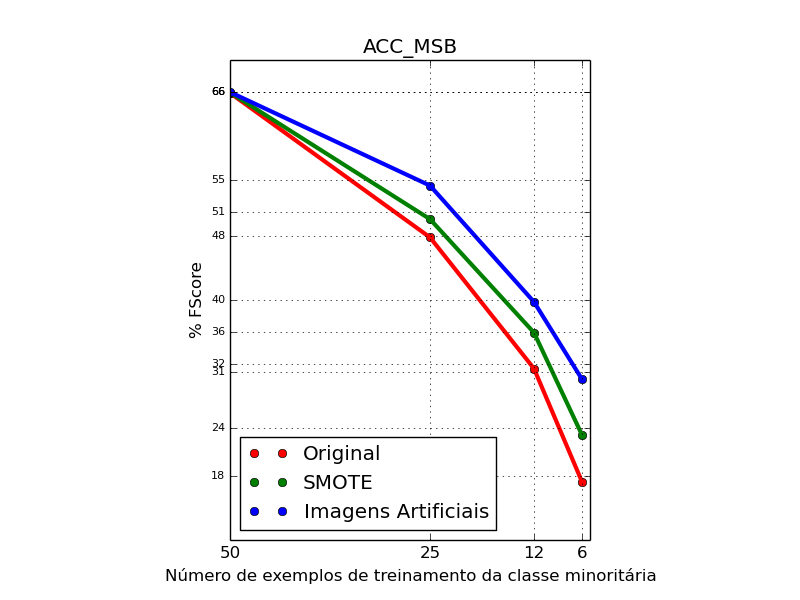
\includegraphics[width=\linewidth]{\detokenize {figuras/resultado-melhor4.png}}
  \caption{Original}
\end{subfigure}
\begin{subfigure}{\textwidth}
  \centering
  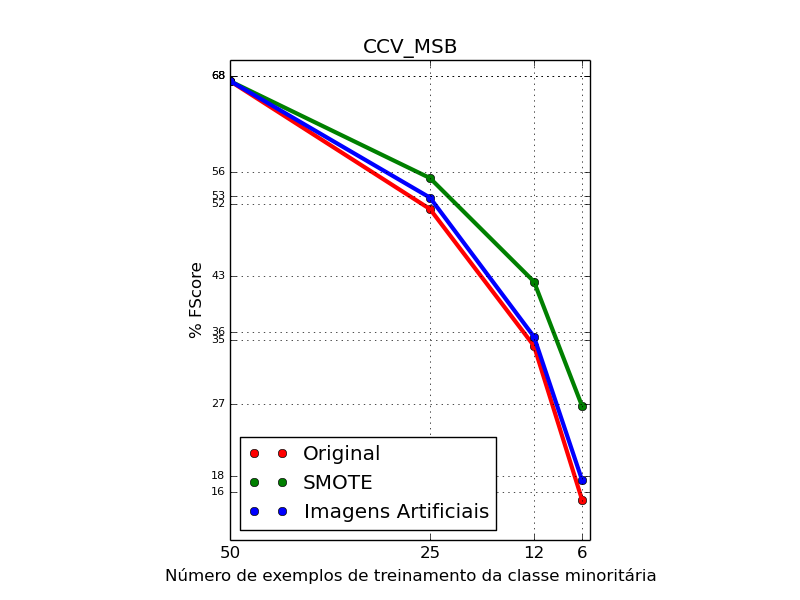
\includegraphics[width=\linewidth]{\detokenize {figuras/resultado-pior1.png}}
  \caption{\textit{Unsharp masking}}
  \label{fig:unsharp}
\end{subfigure}
 \end{center}
\end{figure}

\begin{figure}[htb]
 \begin{center}
   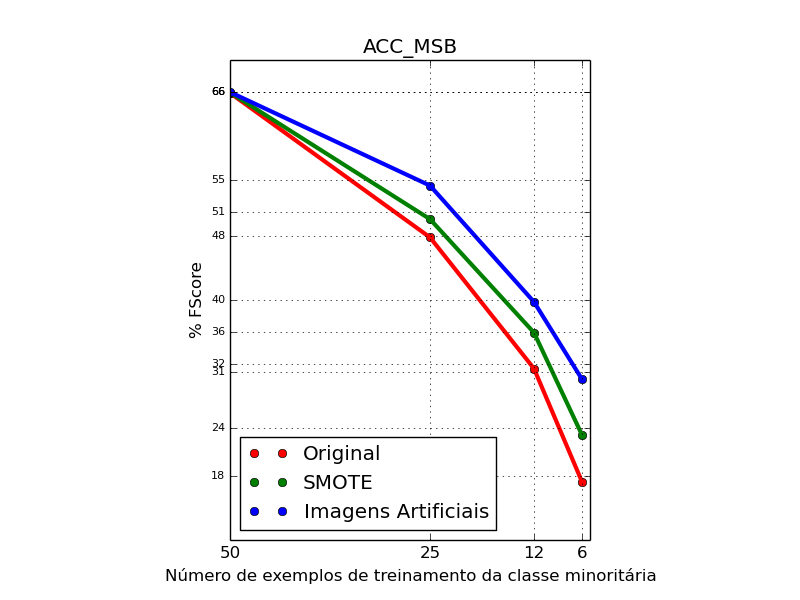
\includegraphics[width=\linewidth]{\detokenize {figuras/resultado-melhor4.png}}
 \end{center}
 \caption[Resultado obtido com a operação de combinação apresentada na Figura~\ref{fig:ArtificialImages}.]{Resultado obtido com a operação de combinação apresentada na Figura~\ref{fig:ArtificialImages}. Apresenta-se a relação da medida-F com a taxa de balanceamento utilizando: as imagens originais, a geração de exemplos com SMOTE e as imagens geradas artificialmente. \textit{Fonte:~Elaborado pelo autor.}}
 \label{fig:resultmelhor}
\end{figure}

\enlargethispage{-1cm}

Também foi possível notar que algumas operações não provocaram a melhora da classificação. A operação de adição de ruído para geração artificial, a posterior extração utilizando CCV e a quantização por MSB, destacou-se como o pior resultado, apresentado na Figura~\ref{fig:resultpior}. Outros casos que não obtiveram o resultado esperado envolveram as operações de borramento e de \textit{unsharp masking}.

\begin{figure}[htb]
 \begin{center}
   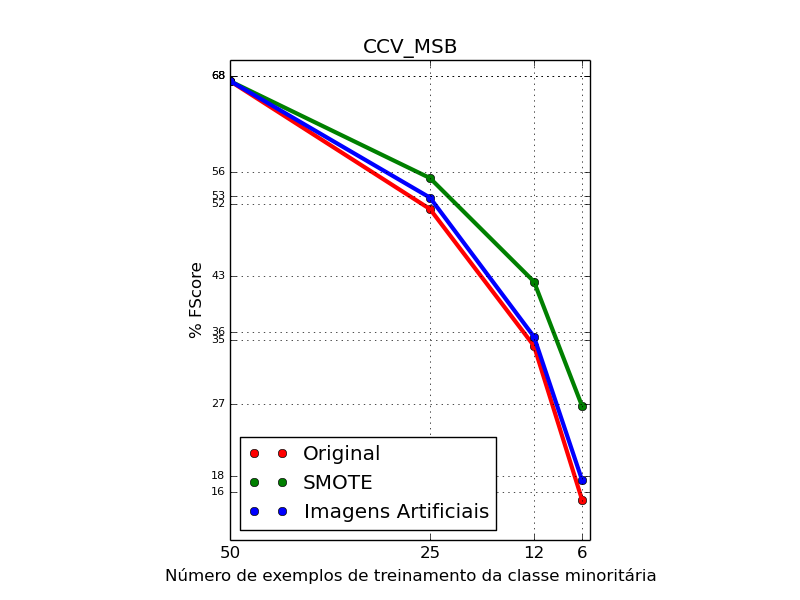
\includegraphics[width=\linewidth]{\detokenize {figuras/resultado-pior1.png}}
 \end{center}
 \caption[Piores resultados, obtidos com a adição de ruído.]{Piores resultados, obtidos com a adição de ruído. Apresenta-se a relação da medida-F com a taxa de balanceamento utilizando as imagens originais, o SMOTE e as imagens artificiais geradas. \textit{Fonte:~Elaborado pelo autor.}}
 \label{fig:resultpior}
\end{figure}

Após a realização dos testes, as operações que melhor se destacaram foram: utilizar todas as operações, apenas mistura e apenas composição. E as operações que resultaram em uma classificação pior do que o uso do SMOTE foram: utilizar apenas borramento, ruído ou \textit{unsharp masking}. Com o teste estatístico de Friedman foi possível verificar que o ACC foi o extrator que melhor se beneficiou das características geradas; e CCV e GCH os menos beneficiados. \enlargethispage{-\baselineskip} A Tabela \ref{tab:result} apresenta os \textit{rankings} encontrados por este teste para todas as execuções das melhores operações. O p-valor computado corresponde a $4.24E^{-11}$, assim a hipótese nula de que não há diferença entre as execuções foi rejeitada. Vale destacar que para algumas execuções, o teste de Friedman retornou o \textit{ranking}: geração artificial (1), SMOTE (2) e imagens originais (3), ou seja, sem que SMOTE e a geração artificial concorressem pela mesma posição, diferente da tabela apresentada.

\begin{table}[htb]
\centering
\caption{Posição média dos algoritmos utilizando Friedman}
  \begin{tabular}{c|c}
    Algoritmos  &   Posição \\ \hline
    Original    &   3.0000  \\
    Smote       &   1.6136  \\
    Artificial  &   1.3863  \\
  \end{tabular}
 \label{tab:result}
\end{table}

Em outro experimento, utilizou-se as cópias das imagens de treino para rebalancear, sem realizar nenhuma operação de pré-processamento (método conhecido como SRS - \textit{Simple Random Sampling}). A Figura~\ref{fig:resultcopia} mostra as respectivas medidas-F encontradas. É possível notar que a cópia dessas imagens não adiciona nenhuma informação nova para o aprendizado.

\begin{figure}[htb]
 \begin{center}
   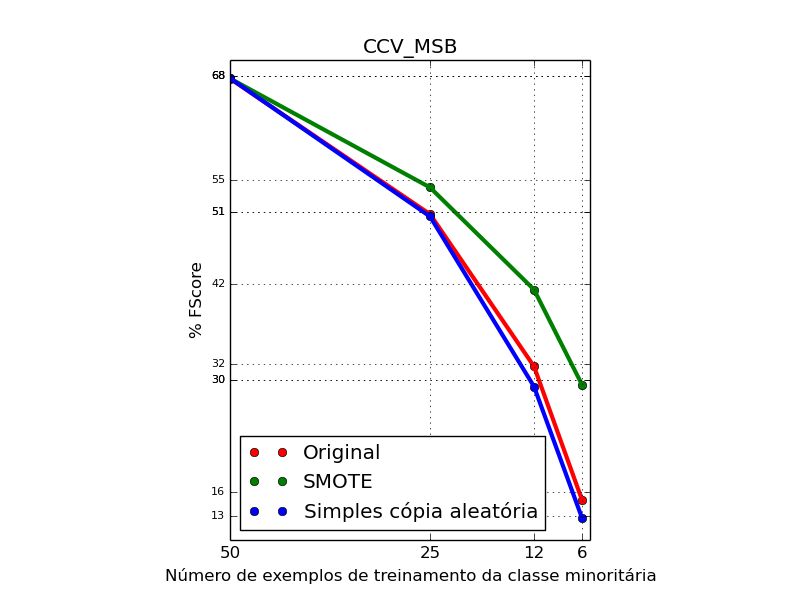
\includegraphics[width=\linewidth]{\detokenize {figuras/resultado-copia.png}}
 \end{center}
  \caption[Simples replicação de exemplos sem realizar nenhuma operação.]{Simples replicação de exemplos sem realizar nenhuma operação de pré-processamento. É possível verificar que não foi adicionada nenhuma informação relevante para o aprendizado. \textit{Fonte:~Elaborado pelo autor.}}
 \label{fig:resultcopia}
\end{figure}
%--------------------------------------------------------------------------------
\section{Trabalhos futuros}

O treinamento de uma rede neural de convolução~\footnote{\url{http://caffe.berkeleyvision.org/}} foi realizado, utilizando as classes ``praia'' e ``montanha'', balanceadas, da base COREL-1000. A classificação sobre este treinamento obteve $\approx 80\%$ de acurácia, enquanto que utilizando os extratores padrões foi possível atingir apenas $\approx 69\%$. Isso reforça a proposta de analisar quais são as características latentes que esse tipo de rede neural consegue extrair. Para essa análise vão ser utilizadas bases discriminadas quanto às propriedades de textura, cor e forma.

Além de analisar o processamento realizado por uma rede de convolução para a classificação das imagens, uma rede RBM também será treinada para análise da sua memória associativa. As imagens artificialmente geradas foram adicionadas no conjunto de treino sem verificação da sua relevância, o que pode ter prejudicado a classificação. A memória associativa aprendida com o treinamento de uma máquina de Bolztmann restrita pode vir a auxiliar no entendimento dessas imagens como relevantes ou não. Além disso, pode servir como escolha para qual imagem original utilizar, ao invés do método aleatório utilizado nos resultados preliminares.


%--------------------------------------------------------------------------------
\section{Considerações finais}

Com os experimentos realizados foi possível notar que a geração de imagens artificiais pode gerar novas informações para a classificação das imagens. O que indica que um estudo mais aprofundado de quais operações podem ser aplicadas nas imagens originais auxilie o cenário de bases desbalanceadas.

Dessa forma, esse capítulo também apresentou as próximas tarefas a serem realizadas. Foi destacada a análise das redes de convolução para identificar quais características latentes são automaticamente extraídas. Apesar de algumas operações de pré-processamento terem gerado imagens que melhoraram a classificação, algumas não causaram melhora. Isso indica que a análise da relevância da informação contida em imagens deve melhorar esse resultado. A memória associativa, aprendida com uma máquina de Boltzmann restrita, deve ser capaz de indicar se uma determinada imagem é relevante para o aprendizado.
